\section{Theory}

\subsection{Kohn-Sham density functional theory}

Kohn-Sham density functional theory, total energy of a system of interacting
electrons can be written as \cite{Kohn1965}:
\begin{equation}
E_{\mathrm{tot}}\left[\{\psi_{i}(\mathbf{r})\},\rho(\mathbf{r})\right] =
E_{\mathrm{kin}} + E_{\mathrm{ion}} + E_{\mathrm{Ha}} + E_{\mathrm{xc}}
\label{eq:KS_ene_func}
\end{equation}
where $\{\psi_{i}(\mathbf{r})\}$ is a set of single-electron wave functions or
Kohn-Sham orbitals
and $\rho(\mathbf{r})$ is electronic density:
\begin{equation}
\rho(\mathbf{r}) = \sum_{i_{st} = 1}^{N_{st}} f_{i_{st}} \psi^{*}_{i_{st}}(\mathbf{r})
\psi_{i_{st}}(\mathbf{r})
\end{equation}

$E_{\mathrm{kin}}$ is kinetic energy of independent electrons described by
Kohn-Sham orbitals:
\begin{equation}
E_{\mathrm{kin}} = -\frac{1}{2}\sum_{i_{st}}
\int f_{i_{st}}
\psi_{i_{st}}^{*}(\mathbf{r})\,\nabla^2\,\psi_{i_{st}}(\mathbf{r})
\,\mathrm{d}\mathbf{r}
\end{equation}
%
$E_{\mathrm{ion}}(\mathbf{r})$ represents ion-electron interaction energy:
\begin{equation}
E_{\mathrm{ion}} = \int V_{\mathrm{ion}}(\mathbf{r})\, \rho(\mathbf{r})\,
\mathrm{d}\mathbf{r}
\end{equation}
%
$E_{\mathrm{Ha}}$ represents energy of classical distribution
of charges (electrons) density which is also known as Hartree energy:
\begin{equation}
E_{\mathrm{Ha}} = \frac{1}{2} \int 
\dfrac{\rho(\mathbf{r})\rho(\mathbf{r}')}
{\left|\mathbf{r} - \mathbf{r}'\right|}
\mathrm{d}\mathbf{r}\mathrm{d}\mathbf{r}'
\end{equation}
%
The last energy term, $E_{\mathrm{xc}}$ is the exchange-correlation energy.
It has several forms, however, in this work we will use on the so-called
local density approximation of $E_{\mathrm{xc}}$:
\begin{equation}
E_{\mathrm{xc}} = \int \epsilon_{\mathrm{xc}}\left[\rho(\mathbf{r})\right]
\rho(\mathbf{r})\,\mathrm{d}\mathbf{r}
\end{equation}

Application of variational principle to energy functional \ref{eq:KS_ene_func}
under the constraint
\begin{equation}
\int \psi^{*}_{i_{st}}(\mathbf{r}) \psi_{i_{st}}(\mathbf{r})\,\mathrm{d}\mathbf{r} = 1
\end{equation}
results in the so-called Kohn-Sham equation:
\begin{equation}
\left[
-\frac{1}{2}\nabla^2  + V_{\mathrm{KS}}(\mathbf{r})
\right] \psi_{i_{st}}(\mathbf{r}) =
\epsilon_{i_{st}}\psi_{i_{st}}(\mathbf{r})
\end{equation}
where $\epsilon_{i_{st}}$ and $\psi_{i_{st}}(\mathbf{r})$ is known as Kohn-Sham
eigenvalues and eigenvectors (orbitals).
Quantity $V_{\mathrm{KS}}$ is called the Kohn-Sham potential, which can be
written as sum of several potentials:
\begin{equation}
V_{\mathrm{KS}}(\mathbf{r}) = V_{\mathrm{ion}}(\mathbf{r}) + V_{\mathrm{Ha}}(\mathbf{r})
+ V_{\mathrm{xc}}(\mathbf{r})
\label{eq:KS-pot}
\end{equation}
%
$V_{\mathrm{ion}}$ denotes attractive potential between ion (or atomic nuclei)
with electrons. This potential can be written as:
\begin{equation}
V_{\mathrm{ion}}(\mathbf{r}) =
\sum_{I}^{N_{\mathrm{atoms}}}
\frac{Z_{I}}{ \left| \mathbf{r} - \mathbf{R}_{I} \right| }
\end{equation}
This potential is Coulombic and has singularities
at the ionic centers. It is generally difficult to describe this potential
numerically, so it is common to replace the full Coulombic potential
with softer potential which is known as pseudopotential.
Note that this potential can also represent any external local potential, for
example harmonic confining potential in quantum dot system.

$V_{\mathrm{Ha}}$ is the classical electrostatic potential or commonly known
as the Hartree potential. It is defined as
\begin{equation}
V_{\mathrm{Ha}}(\mathbf{r}) = \int
\frac{\rho(\mathbf{r}')}
{\mathbf{r} - \mathbf{r}'}\,\mathrm{d}\mathbf{r}',
\end{equation}
Alternatively, Hartree potential can also be obtained via solving Poisson equation:
\begin{equation}
\nabla^{2} V_{\mathrm{Ha}}(\mathbf{r}) = -4\pi \rho(\mathbf{r})
\end{equation}
The last term in Equation \eqref{eq:KS-pot} is exchange-correlation potential.

\subsection{Lagrange basis functions}

Use of Lagrange basis functions in electronic structure calculation is relatively new.
Family:

For a given interval $[0,L]$, with $L>0$, the grid points $x_{i}$
appropriate for periodic Lagrange function are given by:

\begin{equation}
x_{i}=\frac{L}{2}\frac{2i-1}{N}
\end{equation}
with $i=1,\ldots,N$. Number of points $N$ should be an odd number.

The periodic cardinal functions $L_{i}^{\mathrm{per}}(x)$, defined
at grid point $i$ are given by:
\begin{equation}
L_{i}^{\mathrm{per}}(x)=\frac{1}{\sqrt{NL}}\sum_{n=1}^{N}\cos\left(\frac{\pi}{L}(2n-N-1)(x-x_{i})\right).
\label{eq:LF_p_1d}
\end{equation}
The expansion of periodic function in terms of Lagrange functions:
\begin{equation}
f(x)=\sum_{i=1}^{N}c_{i}L_{i}^{\mathrm{per}}(x)
\end{equation}
with expansion coefficients $c_{i}=\sqrt{L/N}f(x_{i})$. When doing
variational calculation, the cofficients $c_{i}$ are the variational
parameters. The actual function values $f(x_{i}$) at grid points
$x_{i}$ is obtained by $f(x_{i})=\sqrt{N/L}c_{i}$. The prefactor
is sometimes abbreviated by $h=L/N$ and is also referred to as scaling
factor.

In this work, we will be using periodic Lagrange functions.

\begin{figure}
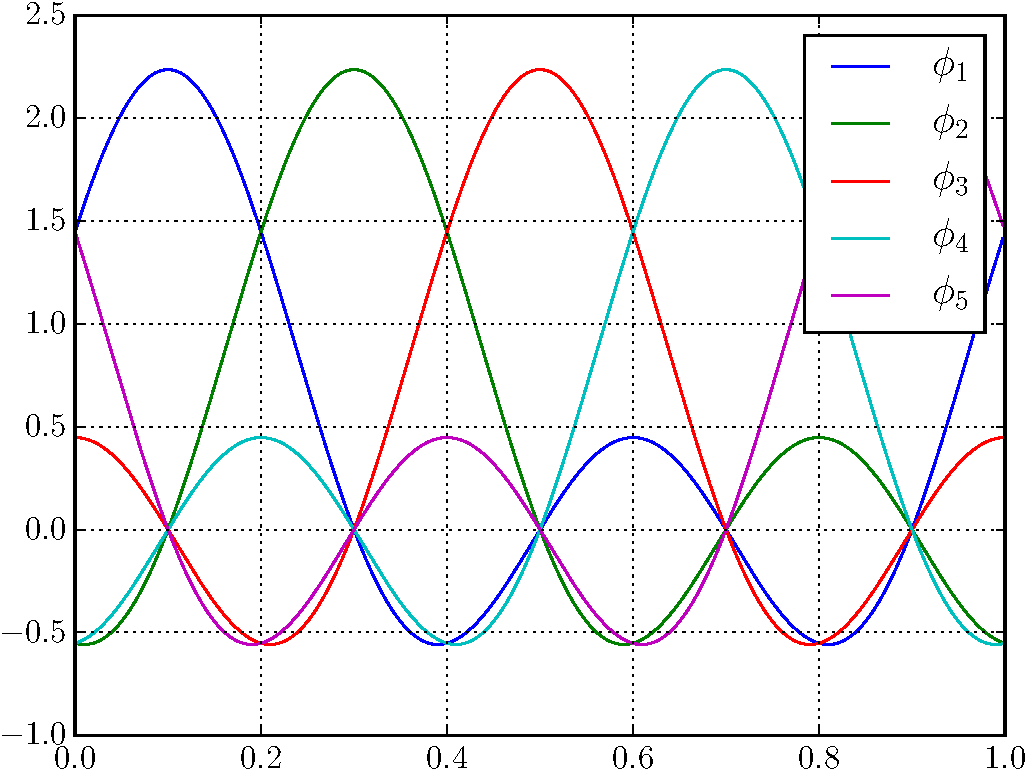
\includegraphics[width=0.5\textwidth]{images/plot_LF_p_N_5.pdf}
\end{figure}

